\documentclass[24pt, a2papper, portrait]{tikzposter}
\usepackage[utf8]{inputenc}
\usepackage{blindtext}
\usepackage{comment}
 
\title{Who to follow on Twitter}
\author{Group 7: POSTER 2}
\date{\today}
\usetheme{Simple}

\begin{document}
\maketitle

\begin{columns}
    \column{0.5}
    \block{Result: tf-idf vs combination (tf-idf and PageRank)} {
        \begin{tikzfigure}
            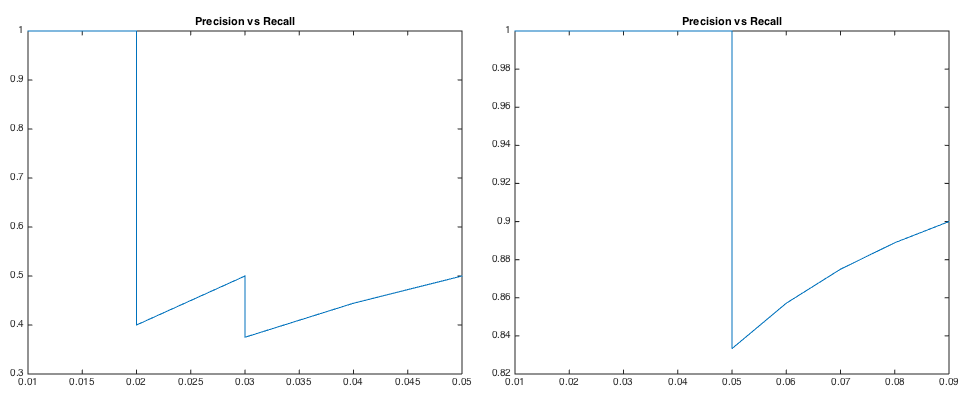
\includegraphics[width=1\linewidth]{images/exptfidf.png}
        \end{tikzfigure}
    }

    \column{0.5}
    \block{Result: PageRank simple vs PageRank weighted by \#followers} {
        \begin{tikzfigure}
            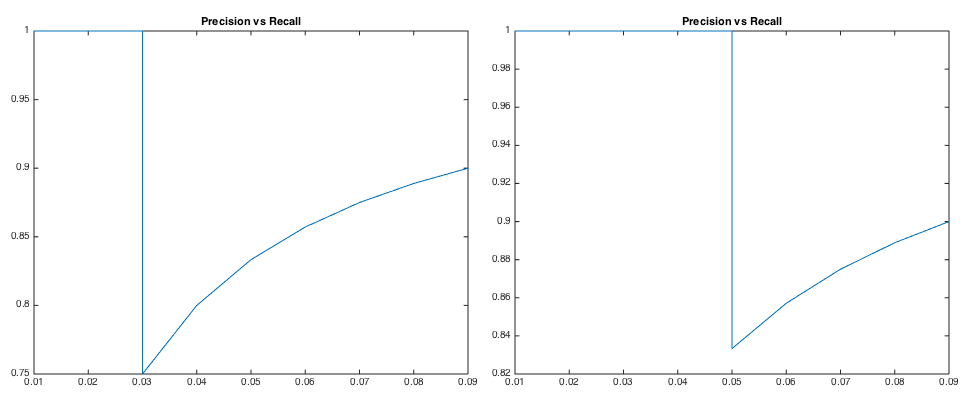
\includegraphics[width=1\linewidth]{images/exptopr.png}
        \end{tikzfigure}
    }
\end{columns}

\begin{columns}
    \column{0.5}
    \block{Conclusion}{
        It is feasible to create a Twitter user recommender engine using tf-idf and
        PageRank. Twitter data is suitable to be represented as a graph. Looking at the
        results, using appropriate parameters for weighing tf-idf and PageRank yields a
        result that is satisfying. Measuring the extent of the satisfaction is
        subjective, but for the group of this project it is deemed that the result is
        satisfactory enough for the given task.

        Due to the limited amount of data and the fact that the data is collected using
        a limited set of correlated hashtags, it is hard to predict if the results are
        applicable to a larger more representative dataset. It would perhaps be better
        to use a larger dataset with tweets from several different topics. However, 
        considering the limited amount of time and resources, the project showed
        that the task is feasible.
    }

    \column{0.5}
    \block{}{}
\end{columns}

\end{document}
